% $Id: gdprefs.tex 11355 2010-06-16 14:48:31Z alexandra $
%ID:prefPageBasicContextId
% Local Variables:
% ispell-check-comments: nil
% Local IspellDict: american
% End:
% --------------------------------------------------------
% User documentation
% copyright by BREDEX GmbH 2004
% --------------------------------------------------------
\index{Preferences!GUIdancer}
\index{GUIdancer!Preferences}
\label{gdprefs}

\begin{figure}[h]
\begin{center}
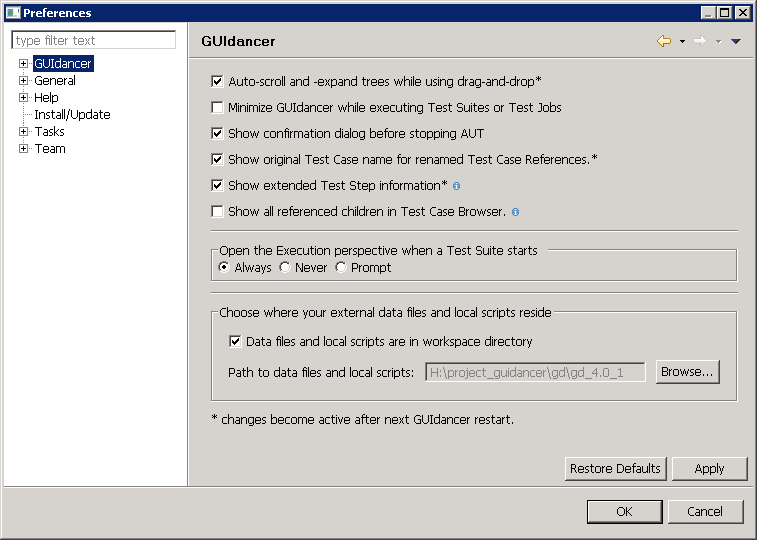
\includegraphics[width=12.5cm]{Tasks/Preferences/PS/gdprefs}
\caption{\jb{} Preference Dialog}
\label{gdprefs}
\end{center}
\end{figure}

 From this page, you can configure your preferences for:
\begin{description}
\item [Auto-scrolling and -expanding:]{When the checkbox is marked, the views and browsers in \jb{} automatically scroll in the direction you move the mouse when you are dragging and dropping. Trees will also be automatically expanded when you hover over them while dragging items.}
\item [Minimizing \jb{}:]{When the checkbox is marked, \jb{} is automatically minimized when test execution begins. This is useful if you are letting tests run on the same machine you are specifying on.}
\item [\gdaut{} confirmation dialog:]{When the checkbox is marked, a dialog appears to check if you are sure when you click the  \bxcaption{stop \gdaut{}} button.}
\item [Original \gdcase{} name:]{When the checkbox is activated, you can see the original name of a referenced \gdcase{} in brackets behind a new name you enter for the \gdcase{}. This can help you to see and search for \gdcases{} you have reused. }
\item[\gdstep{} information:]{When this checkbox is activated, you see the details about the \gdstep{} (the component name and type, and the action) in square brackets behind the \gdstep{} name. If you do not want to see these details, you can deactivate this checkbox.}
\item[Show referenced children:]{When this option is not active, you can only see  referenced parent \gdcases{} in the \gdtestcasebrowser{}. The referenced \gdcases{} contained in these \gdcases{} are not displayed. This action can be useful if you want to improve the speed of working with the \jb{} client.}
\item [Switching to the Execution perspective:]{When the test begins, \jb{} can automatically change to the Execution perspective. You can choose to always be asked, to always change, or to never change. }
\item [Data files location:]{You can specify a location where external data files (e.g. Excel files) are held, or use the workspace directory as the base location. }
\bxtipp{The advantage of using the workspace as a location for your data files is that you can view these in the navigator view directly in \jb{}. Windows users can even open Excel files in \jb{} using the In-Place editor.}
\end{description}

 

